\documentclass[tikz,border=6pt]{standalone}
\usepackage{amsmath,amssymb}
\usepackage{xcolor}
\definecolor{accent}{HTML}{A13D2C}
\definecolor{accent2}{HTML}{2B5F6B}
\definecolor{muted}{HTML}{5A564F}
\definecolor{linecol}{HTML}{D8D2C4}
\definecolor{astroblue}{HTML}{1B4F72}
\definecolor{sunyellow}{HTML}{E8A33D}
\usetikzlibrary{calc,arrows.meta}
\usepackage[T1]{fontenc}\usepackage{newpxtext,newpxmath}  % same fonts as the notes
\begin{document}
% Point-lens light curves, all analytic:
%   u(t) = sqrt(u0^2 + tau^2), tau = (t - t0)/tE,   A(u) = (u^2+2)/(u sqrt(u^2+4))   (ga:eq:magnification)
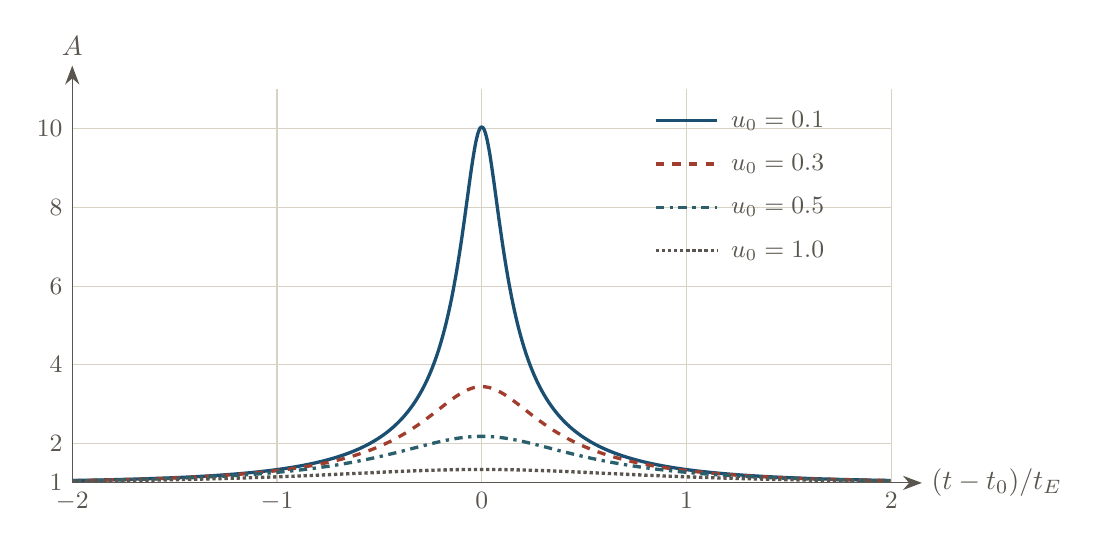
\begin{tikzpicture}[x=2.6cm,y=0.5cm, >={Stealth[length=2.4mm]}]
  \foreach \y in {2,4,...,10} \draw[linecol] (-2,\y) -- (2,\y);
  \foreach \x in {-2,-1,0,1,2} \draw[linecol] (\x,1) -- (\x,11);
  \draw[->, muted] (-2,1) -- (2.15,1) node[right] {$(t-t_0)/t_E$};
  \draw[->, muted] (-2,1) -- (-2,11.6) node[above] {$A$};
  \foreach \x in {-2,-1,0,1,2} \node[below, muted] at (\x,1) {\small $\x$};
  \foreach \y in {1,2,4,6,8,10} \node[left, muted] at (-2,\y) {\small \y};
  % one curve per impact parameter u0
  \foreach \uo/\col/\sty/\n in {0.1/astroblue/solid/801, 0.3/accent/dashed/401, 0.5/accent2/dash dot/301, 1.0/muted/densely dotted/201}{
    \draw[\col, line width=1.2pt, \sty, domain=-2:2, samples=\n]
      plot (\x, {((\uo*\uo+\x*\x)+2)/(sqrt(\uo*\uo+\x*\x)*sqrt(\uo*\uo+\x*\x+4))});
  }
  % legend
  \begin{scope}[shift={(0.85,10.2)}]
    \foreach \uo/\col/\sty/\k in {0.1/astroblue/solid/0, 0.3/accent/dashed/1, 0.5/accent2/dash dot/2, 1.0/muted/densely dotted/3}{
      \draw[\col, line width=1.2pt, \sty] (0,-1.1*\k) -- (0.3,-1.1*\k);
      \node[right, muted] at (0.32,-1.1*\k) {\small $u_0=\uo$};
    }
  \end{scope}
\end{tikzpicture}
\end{document}
